\begin{center}
    \textbf{--------- Lezione 3 - 8 marzo 2021 ---------}
\end{center}
\section[Stima della posizione con dati soggetti a rumore]{Stima della posizione con dati soggetti a \\rumore}
In diversi contesti si ha il problema che devo stimare un valore o lo stato di un sistema come ad esempio l'angolo di pitch di un aereo (angolo che assume la pala rispetto al piano di rotazione del rotore). 
Si ha anche il problema che il calcolo deve essere effettuato sulla base di varie misurazioni soggette a rumore, come ad esempio accelerometri installati in varie parti dell'aereo. 

Applichiamo il problema all'indoor positioning, andiamo quindi a stimare la posizione di un utente. 
Ci sono alcuni spostamenti che non sono possibili, ci facciamo aiutare dalla planimetria, ad esempio un utente non può passare attraverso i muri oppure non può salire su un piano superiore se non ci sono scale o ascensori. 

\subsection{Modello bayesiano}
Abbiamo una serie di osservazioni $z_1$...$z_n$ che rappresentano le osservazioni nel tempo.
\\ Vogliamo calcolare B($x_t$), dove B sta per belief, che rappresenta la certezza che la posizione al tempo t sia x. 
Abbiamo quindi che 
\begin{center}
    B($x_t$) = P($x_t$ $|$ $z_1...z_n$)
\end{center}
Nel modello, la B($x_t$) dipende da tutte le osservazioni possibili. 
Siccome è una distribuzioni di probabilità, la somma per tutte le x di B($x_t$) è 1. 
\\ Il modello bayesiano è generico ma non ci indica come calcolare la soluzione. 

\subsection{Modello Markoviano}
Nel modello bayesiano è difficile calcolare una soluzione perchè la valutazione dipende da tutta la storia delle osservazioni. 

C'è un modello meno espressivo che permette di rappresentare una sottoclasse di problemi, il modello markoviano. 
È più semplice dal punto di vista formale e di calcolo, ma ha un'espressività tale da permettere di modellare la maggior parte dei problemi di interesse pratico in questo campo. 
Assumiamo che la posizione al tempo t (cioè B($x_t$) per tutte le $x_t$) dipenda solo dal valore di belief al tempo t-1, cioè B($x_{t-1}$) e dal valore di $z_t$.
\\ In pratica non mi interessano tutte le misurazioni ma l'ultima osservazione al tempo t-1. 

\subsection{Modello di transizione di stato (o modello di spostamento)}
Il modello di transizione di stato mi permette di capire dove io posso essere al tempo t data la mia posizione al tempo t-1. 
\\Ero da qualche parte in t-1, dove potrei essere al tempo t?
\\$B^-$($x_t$) rappresenta la probabilità di dove si trovi l'utente al tempo t tenendo in considerazione che so dov'era al tempo t-1. 
\\$B^-$($x_t$) dipende da B($x_{t-1}$) e dalla probabilità P($x_t$  $|$ $x_{t-1}$) che ci sia stato uno spostamento tra $x_{t-1}$ e $x_t$. 

Esempi:
\begin{itemize}
    \item la distanza tra $x_{t-1}$ e $x_t$ è 20 metri e la distanza tra t-1 e t è di 5 secondi. Considerando che l'utente sia a piedi, è improbabile che l'utente abbia percorso quella distanza in così poco tempo, quindi il valore della probabilità P($x_t$ $|$ $x_{t-1}$) sarà basso ma non zero. Può essere che l'utente stesse correndo
    \item al tempo t-1 gli unici valori di $x_{t-1}$ per i quali B($x_{t-1}$) è non-zero sono al primo piano. 
    Al tempo t considero una $x_t$ al secondo piano e non ci sono né scale né ascensori lì vicino. La distanza temporale tra t-1 e t è di 5 secondi. $B^-$($x_t$) sarà zero perché è impossibile che un utente passi da un piano all'altro in così poco tempo non avendo scale o ascensore
    \item consideriamo uno spazio dimensionale e tre posizioni nel tempo t-1: $x^a$,$x^b$,$x^c$. 
    \\ Con B($x^a$) = 1/2, con B($x^b$) = 1/6, con B($x^c$) = 2/6.
    \begin{itemize}
        \item P($x_t$ $|$ $x^a$) = 0, la probabilità che un utente si muova da $x^a$ ad $x_t$ è 0 perchè la distanza è troppa 
        \item P($x_t$ $|$ $x^b$) = 0,1, è possibile ma improbabile, l'utente deve essere andato molto velocemente
        \item P($x_t$ $|$ $x^c$) = 0,5 è probabile nel mio modello
    \end{itemize}
    \begin{center}
        \begin{math}
        B^- (x_t) = \frac{1}{2}*0+\frac{1}{6}*0,1+\frac{2}{6}*0,5
        \end{math}
    \end{center}
\end{itemize}
\begin{center}
    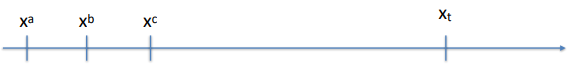
\includegraphics[width=.9\textwidth]{images/MobiDEV/2. tecniche di aggregazione di dati soggetti a rumore/modello di transizione di stato.PNG} \\
\end{center}

\subsection{Modello percettivo}
Prende in considerazione l'osservazione che abbiamo fatto. 
Vogliamo stimare quanto è la probabilità che in $x_t$ percepiamo $z_t$. Non stiamo stimando il punto ma la probabilità di percepire quella certa osservazione.
\\ Esempio: $z_t$ è un alto valore di RSSI rispetto ad un beacon bluetooth:
\begin{itemize}
    \item $x_t^1$ è una posizione a 100 metri dal beacon, quindi P($z_t$ $|$ $x_t^1$) = 0, questo perchè il beacon non può essere percepito a 100 metri di distanza
    \item $x_t^2$ è una posizione a 1m dal beacon, quindi P($z_t$ $|$ $x_t^2$) sarà un valore più alto, certamente non zero 
\end{itemize}

Esempio del sensore e della porta:
abbiamo uno spazio mono-dimensionale, c'è un sensore che ti avvisa quando sei vicino ad una porta, ma non sai a quale porta. Le osservazioni $z_t$ sono del tipo "sei vicino ad una porta".
In qualche modo il sistema sa anche come si sta spostando l'utente. 

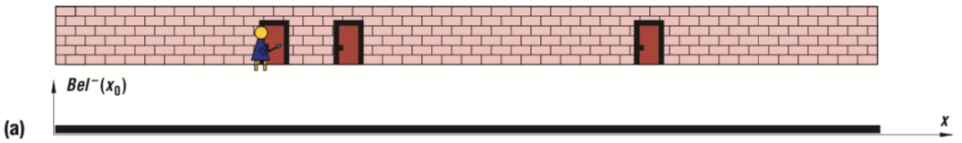
\includegraphics[width=\textwidth]{images/MobiDEV/2. tecniche di aggregazione di dati soggetti a rumore/modello percettivo 1.PNG} \\
Il Bel- mi indica il Belief prima di effettuare l’osservazione. In questo caso, non ho nessuna storia dell’osservazione quindi l’individuo potrebbe essere in qualsiasi parte della stanza: la distribuzione è uniforme. \\
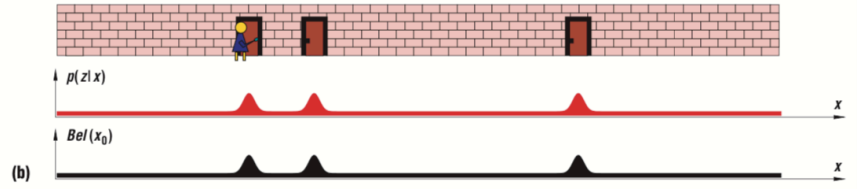
\includegraphics[width=\textwidth]{images/MobiDEV/2. tecniche di aggregazione di dati soggetti a rumore/modello percettivo 2.PNG}
Alla prima osservazione sappiamo che abbiamo una probabilità più alta di essere vicino ad una porta. Il sensore può sbagliare, dunque la probabilità lontano da una porta è bassa, ma non zero.
In questo caso B($x_0$) coincide con p(z $|$ x) perché la distribuzione precedente B-($x_0$) è uniforme \\
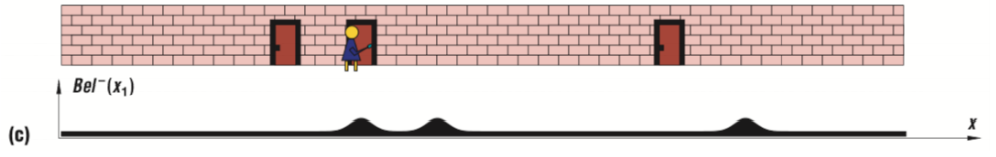
\includegraphics[width=\textwidth]{images/MobiDEV/2. tecniche di aggregazione di dati soggetti a rumore/modello percettivo 3.PNG}
Il sistema poi percepisce che l'utente si è spostato e confronta i picchi con quelli precedenti. I picchi sono meno marcati perché anche nell'osservazione dello spostamento ci possono essere degli errori. \\
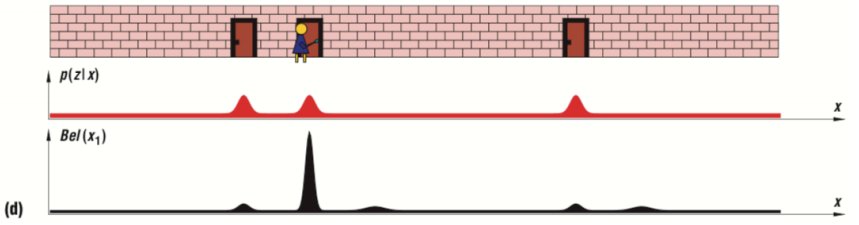
\includegraphics[width=\textwidth]{images/MobiDEV/2. tecniche di aggregazione di dati soggetti a rumore/modello percettivo 4.PNG}
Quando viene fatta la seconda osservazione, p(z $|$ x) non cambia rispetto a prima.
\\ B($x_1$) viene calcolato partendo da una distribuzione precedente non uniforme, otteniamo un picco alto dove un picco su p(z $|$ x) coincide con un picco $B^-$1($x_1$).

\section{Calcolo della posizione adottando il modello Markoviano}
Allargando lo spazio il costo computazionale aumenta.
\\ Per applicare il modello markoviano dobbiamo specificare come calcolare: 
\begin{itemize}
    \item il modello di transizione di stato, dipende da molti fattori come ad esempio il modo di spostamento dell'utente, la mappa dell'ambiente, l'adozione di sistemi inerziali per il calcolo dello spostamento
    \item il modello percettivo, dipende principalmente da quali tecnologie di posizionamento stiamo adottando
\end{itemize}

Esistono vari approcci per calcolare il modello di transizione e percettivo: 
\begin{itemize}
    \item filtro di Kalman
    \item sistemi discreti che rappresentano lo spazio come una griglia o un grafo
    \item particle filter
\end{itemize}

Una delle difficoltà, dal punto di vista computazionale, deriva dal fatto che lo spazio sia una dimensione continua.
\\ Le soluzioni basate sul filtri di Kalman si adattano al dominio continuo, forniscono una soluzione esatta e necessitano di alcune assunzioni sul problema stesso che spesso non valgono per il calcolo della posizione.

\subsection{Approccio basato su griglia}
Discretizzo (trasformo le dimensioni continue dello spazio in discontinue) lo spazio attraverso una griglia che copre l'intera area. \\ Immaginiamo di avere una griglia 3D, oppure un insieme di griglie 2D, una per piano. 
\\ Ogni elemento della griglia è una cella. 
\\ All'inizio B(x) è uniforme per tutte le celle x, ciò significa che non so dove si possa trovare l'utente. 
\\ Per ogni coppia di celle x1, x2 e per una distanza temporale $\Delta$t, posso calcolare la probabilità p($x1_t$ $|$ $x2_{t-1}$) di essere in x1 al tempo t, condizionata dal fatto che ero in x2 al tempo t-1. 
\\ Questo calcolo può tener conto di:
\begin{itemize}
    \item distanza spaziale e temporale
    \item un'osservazione di spostamento, ad esempio l'utente è rimasto fermo, oppure si è spostato per circa x metri in una direzione, ecc.)
    \item della struttura dell'ambiente, ad esempio l'utente non può attraversare i muri
\end{itemize}

Dato $B^-$($x_t$), per ottenere $B^+$($x_t$) mi serve calcolare P($z_t$ $|$ $x_t$).
Per ogni cella x posso valutare la probabilità di fare l’osservazione $z_t$.
\\ Ovviamente devo tener conto della tipologia di osservazione (segnale radio, riconoscimento di un marcatore, ecc.)
Posso farlo perché ho un numero finito di celle.
Dato $B^+$($x_t$) è semplice normalizzare e ottenere B(x).

Assumiamo che per ogni coppia di x1, x2 il calcolo di P($x1_t$ $|$ $x2_{t-1}$) richieda tempo costante e che per ogni cella x, il calcolo di  P($z_t$ $|$ $x_t$) richiede tempo costante.
Allora ottengo, dato n il numero di celle:
\begin{itemize}
    \item Spostamento O(n2)
    \item Percezione: O(n)
\end{itemize}
Abbiamo una complessità totale: O(n2)
\\ La complessità computazionale potrebbe essere maggiore, se ho complessità non costante per calcolare  P($x1_t$ $|$ $x2_{t-1}$) e P($z_t$ $|$ $x_t$) 

Fino ad ora abbiamo assunto di voler tenere traccia della posizione dell'utente, dunque abbiamo 3 dimensioni. 
Se volessimo tener traccia dell'orientamento, potremmo considerare l'orientamento come unico valore (la direzione in cui sta puntando l'utente, mentre si muove sul piano) anche se in alcuni contesti ci serve un orientamento a 3 dimensioni (i 3 angoli con i quali è orientato il dispositivo).
Possiamo discretizzare la rotazione e avere altre 3 dimensioni:
\begin{itemize}
    \item in questo caso dobbiamo avere una cella per ogni combinazione di posizione (3 dimensioni) e rotazione (altre 3 dimensioni)
    \item il numero di celle cresce esponenzialmente con il numero di dimensioni
\end{itemize}

In termini pratici vogliamo che le celle siano piccole, perché devono rappresentare la posizione/orientamento e se fossero troppo grandi non sarebbero precise. 
\\ Questa tecnica può andare bene in alcuni casi, caratterizzati da almeno alcuni di questi fattori:
\begin{itemize}
    \item sono interessato solo a poche dimensioni
    \item ambienti di piccole dimensioni
    \item non ho bisogno di grande precisione, dunque posso usare celle più grandi
    \item gli aggiornamenti sono discontinui e ho elevata potenza di calcolo
\end{itemize}

\section{Particle filter (Sequential Monte Carlo)}
È una tecnica utile per calcolare la posizione secondo il modello Markoviano che calcola una soluzione approssimata, come per le griglie con la differenza che permette di gestire meglio il problema della discretizzazione dello spazio. 
\\ Facciamo tante ipotesi, ciascuna associata ad un peso (probabilità di quell'ipotesi). 
\\ Ogni coppia $<$ipotesi, peso$>$ è chiamata particella. 
\\ È più facile vedere le particelle come punti nello spazio.
\\ La particella non rappresenta solo la posizione ma potrebbe anche includere anche l'orientamento.

\subsection{Funzionamento}
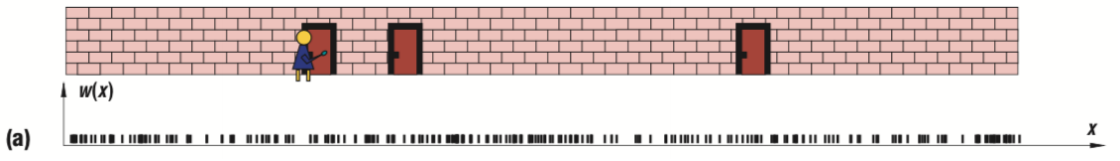
\includegraphics[width=\textwidth]{images/MobiDEV/2. tecniche di aggregazione di dati soggetti a rumore/particle filter 1.PNG}
All'inizio non sappiamo dove sia l'utente, le particelle vengono disposte a caso ed hanno tutte un peso uguale. \\
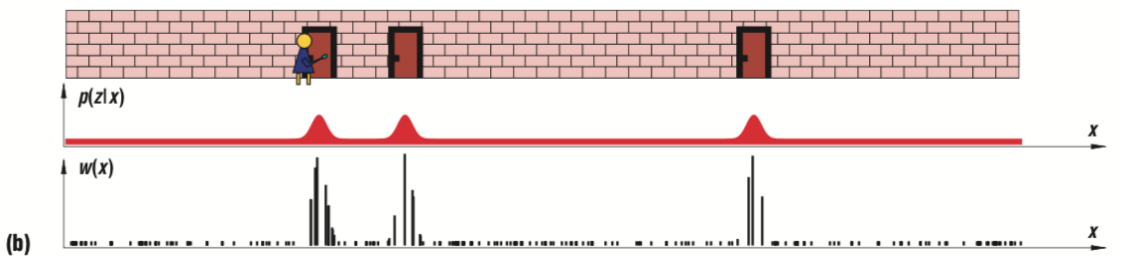
\includegraphics[width=\textwidth]{images/MobiDEV/2. tecniche di aggregazione di dati soggetti a rumore/particle filter 2.PNG}
Quando arriva un'osservazione, cambiamo il peso di ogni particella e lo rendiamo proporzionale alla funzione di probabilità. \\
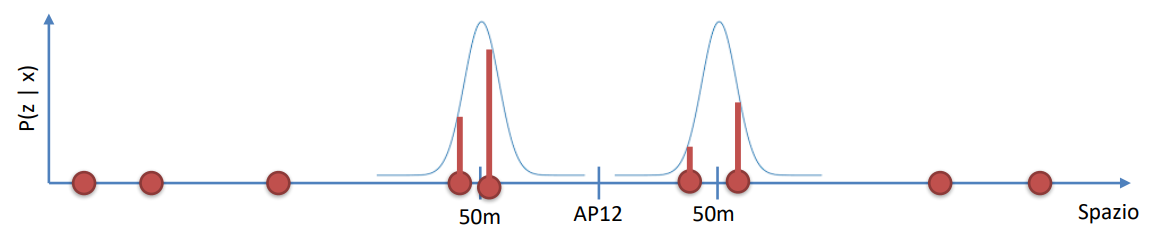
\includegraphics[width=\textwidth]{images/MobiDEV/2. tecniche di aggregazione di dati soggetti a rumore/particle filter_.PNG}
Ad esempio, abbiamo 9 particelle sparse nello spazio e percepisco l'antenna WiFi con AP12. 
\\ Data la potenza del segnale stimo di essere all'incirca a 50 metri di distanza dall'antenna, ma sappiamo che ci potremmo sbagliarci. 
\\ Assegno alla particelle un peso uguale a quello della gaussiana, cioè un valore molto basso, praticamente nullo alle particelle che non si trovano vicino ai 50m di distanza dall'AP. \\
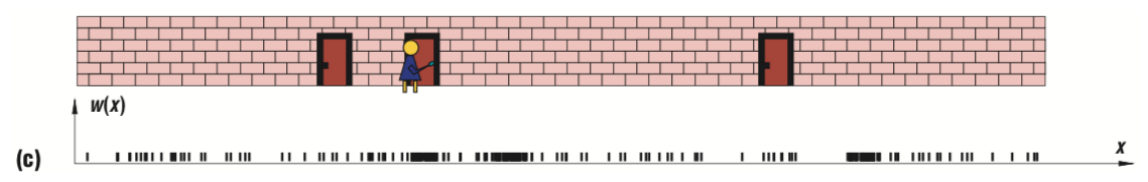
\includegraphics[width=\textwidth]{images/MobiDEV/2. tecniche di aggregazione di dati soggetti a rumore/particle filter 3.PNG}
Quando osservo uno spostamento, creo un nuovo insieme di particelle P', ma il numero di particelle rimane uguale e tutte quante le particelle hanno lo stesso peso. 
\\ Le particelle vengono create così: parto da una particella esistente, ne scelgo una a caso pesata rispetto alla probabilità: ho maggiore probabilità di scegliere quella alta rispetto a quella bassa. 
Vediamo meglio come funziona il calcolo dello spostamento.
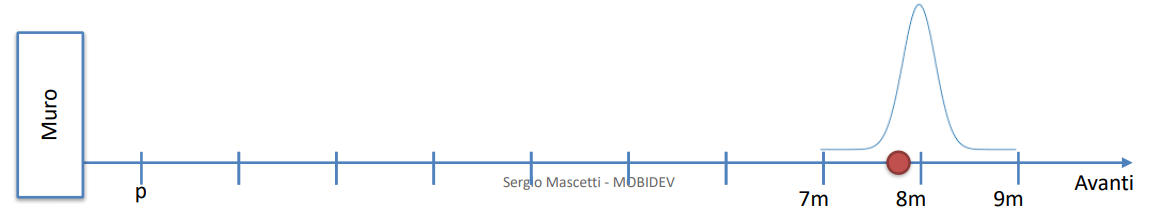
\includegraphics[width=\textwidth]{images/MobiDEV/2. tecniche di aggregazione di dati soggetti a rumore/particle filter_2.PNG}
Abbiamo 1D, contiamo che l'utente fa 10 passi tutti nella stessa direzione, non sappiamo se avanti o indietro.
\\ Partiamo da p, dalla planimetria si che l'utente non può camminare indietro perché c'è il muro, può andare solo avanti. 
\\ Sappiamo che un passo è lungo circa 80 cm (ma potremmo sbagliarci) e stimiamo dove potrebbe arrivare. In questa stima scegliamo poi un punto. 
In pratica modelliamo la probabilità di arrivare in un dato punto con una gaussiana. 
\\ Scegliamo un punto di arrivo casuale all'interno della gaussiana seguendo la probabilità della gaussiana stretta. Il puntino rosso rappresenta la posizione di p'.
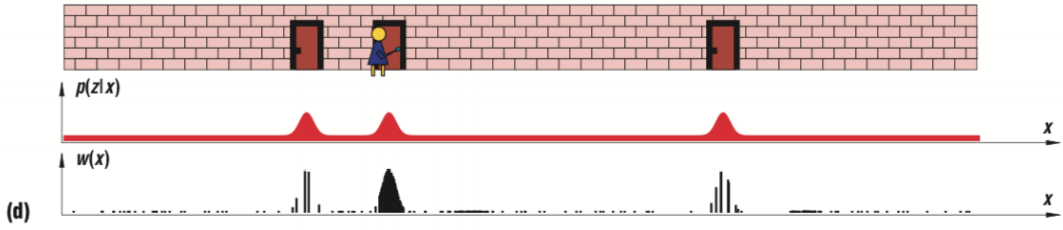
\includegraphics[width=\textwidth]{images/MobiDEV/2. tecniche di aggregazione di dati soggetti a rumore/particle filter 4.PNG}
Quando ottengo una nuova osservazione, modifico il peso delle particelle secondo il modello percettivo. Alla prima porta e alla terza ho una bassa densità di particelle perché lo spostamento non era previsto qua. 
Dove invece era previsto lo spostamento, ho alta densità di particelle.
 
\subsubsection{Quanta incertezza abbiamo?}
Più incertezza modelliamo (cioè più è larga la nostra gaussiana), più lentamente il nostro sistema andrà a convergere, ma siamo più robusti rispetto agli errori.
Se modelliamo meno incertezza (gaussiana più stretta, al limite estremo valore 1 solo per la distanza esatta di 10m), convergiamo prima, ma rischiamo di modellare casi errati, che potrebbero portarci a 
non convergere affatto.
Con meno incertezza c'è il rischio che siccome le particelle tendono a spostarsi dove credono che sia la soluzione corretta, se in caso di errore convergono tutte verso una soluzione errata ad un certo punto tutti i pesi vanno a zero.
Per prevenire questi casi, ad ogni iterazione si possono aggiungere  delle particelle in posizione casuale.

\subsubsection{Quante particelle servono?}
Maggiore è il numero di particelle, meglio riesco a rappresentare il problema. 
Più è grande il numero di particelle più la complessità computazionale cresce. 
Al crescere delle dimensioni devo far crescere il numero delle particelle. 
Ad ogni iterazione calcolo circa 1000 particelle. 

Sia l'approccio basato su griglie che il particle-filtering adottano una forma di discretizzazione dello spazio.
Nell'uso delle griglie discretizzo lo spazio in modo costante e la complessità varia in base alla precisione che uso nel 
rappresentare lo spazio.
Nel particle filter, invece la discretizzazione avviene in termini di particelle: approssimo la posizione (vera) dell'utente a quella di una particella (o di un gruppo di particelle).
\\ La discretizzazione avviene in termini di particelle: approssimo la posizione (vera) dell’utente a quella di una particella (o 
di un gruppo di particelle)
\\ Le particelle a differenza delle celle si spostano, là dove ci sono maggiori probabilità che ci sia l’utente avrò un numero 
più alto di particelle, dunque una discretizzazione più fine dello spazio.


\subsubsection{Implementazione}
Ci sono molte situazioni in cui devo stimare lo stato di un sistema sulla base di più dati soggetti a rumore. 
Il particle filter è una tecnica robusta, generalmente efficiente e abbastanza semplice da implementare. 
Permettono al programmatore di definire delle primitive per 
implementare il modello di spostamento e quello percettivo per una 
singola particelle. 
Questo è molto più semplice (dal punto di vista concettuale) che 
definire il modello su scala globale al sistema.